% This section provides the necessary context to help the reader understand the remainder of the thesis.

% Why this report is generated

As per the PwC survey on crime and fraud we can see that companies who invested money in fraud prevention had to pay 16\% fewer fines and\/ or penalties than those who didn't~, as shown in figure~\ref{fig:fraud_preven}. Hence to protect financial and reputation losses, the companies have to invest money and effort. However, the existing process is costly and human-intensive. The paper focuses on how a machine learning-based system can help companies to reduce overall operational costs and save financial losses.

This paper aims to perform a data-driven approach to extract relevant data to build a machine learning classification model to detect specious companies for a leading trade credit insurance provider. The trade-credit insurance protects the business (customer of the insurance company) in the event their buyers fail to pay for the products or services. Considering the growth of fraudulence cases in the recent past, the insurance provider has to monitor each buyer extensively before approving any insurance policy. 

\begin{figure}[htp]
    \centering
    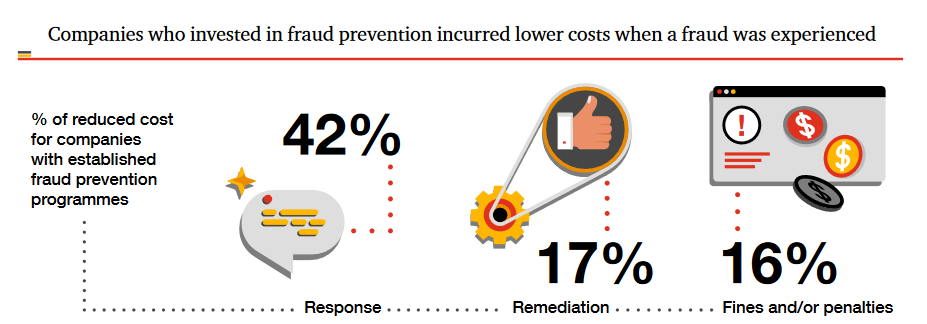
\includegraphics[width=\linewidth]{figures/prevent_fraud.PNG}
    \caption{Investment on Fraud Prevention. Source: PwC 2020 Fraud survey~\cite{PwC.Crime.Survey} }
    \label{fig:fraud_preven}
\end{figure}



\subsection{Trade Credit Insurance}\label{subsec:trade-credit-insurance}
In the business world of trade credit, it is a regular practice to take insurance by manufacturers, suppliers, and service providers to protect their financial interests from any types of risks. Companies sell their products and goods on credit to their buyers. Generally, this is a continuous process as back to back trade deals and payments between the suppliers and buyers. However, the total amount of trade credits are very high. Hence suppliers like to protect their interests by taking credit policies from financial institutions 


For financial institutions (credit insurance provider) ensures financial support to the supplier (their client) in event of any mishaps. Trade credit is a risky business, hence there is an intensive approval process done by the insurance company. As part of the review supplier, buyers, products, sectors, global economic conditions, external factors are checked. As mentioned in section~\ref{sec: Intro}, due to the increased number of fraud cases, insurance providers have to also monitor fraudulent cases. Below are the types of fraud that happens in the trade credit sector.

\begin{itemize}
    \item \textbf{Buyers Fraud:} At the event the buyers of the goods get financially benefited by not paying the dues intentionally to the suppliers.
    \item \textbf{Client Fraud:} When suppliers, the clients of the insurance company try to get economic gain by doing insurance fraud.
    \item \textbf{Joint Fraud:} When the suppliers and buyers cooperate together to conduct insurance fraud get economic gain.
    \item \textbf{Internal Fraud:} When internal parties from the insurance company colludes with the client and conduct an insurance fraud.
\end{itemize}

In this study we will mainly focus on finding the suspicious buyers to prevent economic mishaps to protect the suppliers and the insurance companies from financial loss.


\subsection{Monitor Credit Policy}\label{subsec:monitor-credit-policy}

\subsubsection{Issuing Trade Insurance}\hspace*{\fill} \\
The trade insurance providers go through a sequence of steps to approve or issue a credit policy to their clients. In figure~\ref{fig:trade_credit}, the process of trade credit issuance is shown. First, the client (supplier) requests a credit policy from the trade credit insurance provider after they get a formal purchase request from their buyer. Based on the client's requests, the credit undertaking team of the insurance provider verifies the client, its buyer, the amount and other respective details of the transactions. If the credit undertaking team find the request legitimate then they inform the internal operation team to issue a policy to the client. In the event the buyer fails to pay back for the goods, the supplier (client) applies for an insurance claim from the service provider. After a thorough investigator, the insurance provider pays the money to the supplier and tries to collect the money from the buyers to reduce its operational loss.

\begin{figure}[htp]
    \centering
    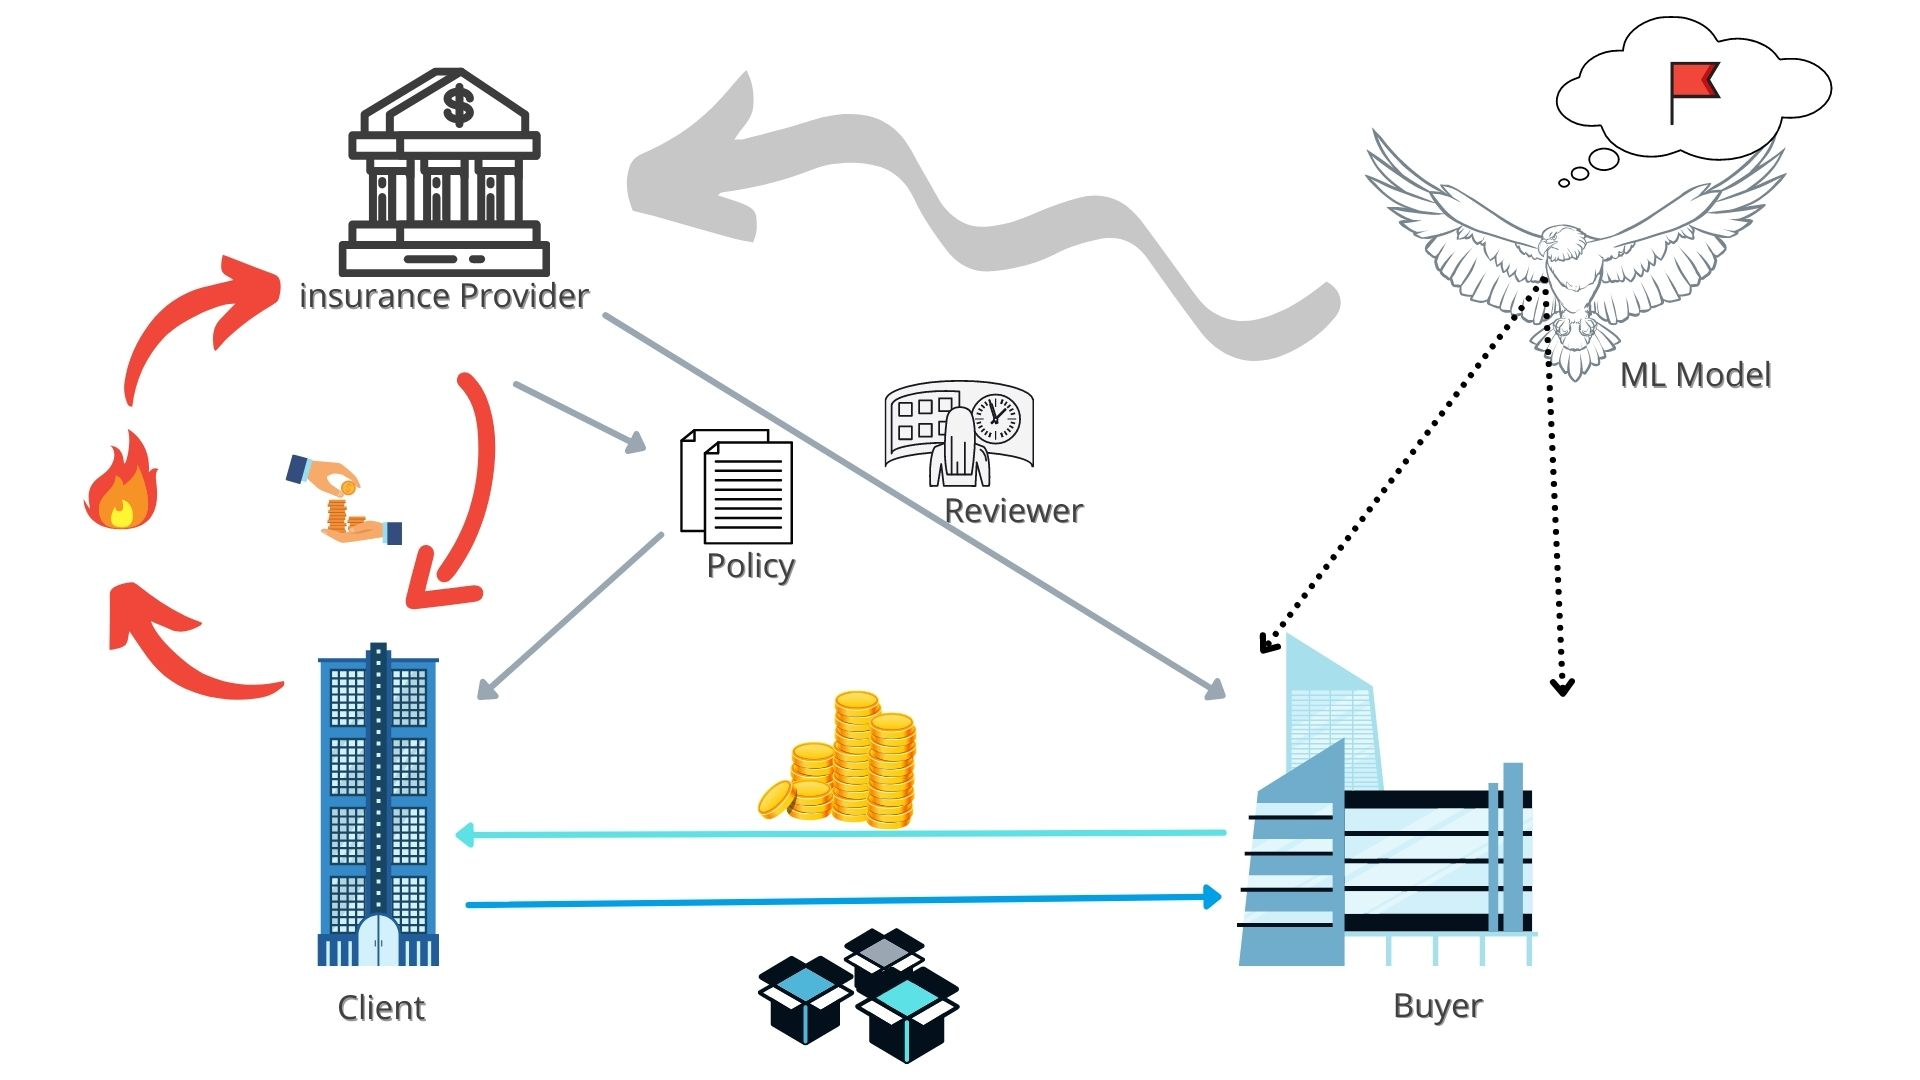
\includegraphics[width=\linewidth]{figures/monitor_buyers.jpg}
    \caption{Trade credit issuing process}
    \label{fig:trade_credit}
\end{figure}


As mentioned earlier in this chapter, there are four different types of fraud that can take place in the trade credit insurance sector. As the report only focuses on the buyers' fraud, only the existing monitoring process and proposed monitoring buyers are mentioned below to identify suspicious events.

\subsubsection{Traditional Approach}\hspace*{\fill} \\
The traditional way of identifying suspicious buyers are done by reviews from the credit undertaking team of the insurance service provider. As mentioned in Section~\ref{sec: Intro} below tools and techniques are currently used by the team.
\begin{itemize}
    \item{Internal System:} The reviews looks for suspicious patterns on the company reports and different system indicators to identify any suspicious companies.
    \item{External System:} The reviews also go through some external links provided by global ALM and regulatory systems to avoid any existing risks.
    \item{Overall Review:} Besides the above system, there are multiple layers of monitoring done by different reviews to reduce operational errors.
\end{itemize}

\subsubsection{Machine learning base Approach}\hspace*{\fill} \\
In the proposed data-driven machine learning technique, a suitable model will be developed based on the data extracted from the different systems by taking input from the experts. Every day the latest policy requests will be fed to the model so that it can predict the highly specious companies. The highlighted companies will be then shared with the credit undertaking team to expedite their reviewing/monitoring process. Based on the outcome and feedback of the reviewer, the model will be continuously updated to improve its performance.



